\chapter{Implementation}
\section{System Architecture and Container Topology}
\textit{SyncFlow} is split into a multi-container web application managed with \textbf{Docker Compose}. Database persistence, backend computation, and static frontend delivery run in separate containers connected over an internal virtual network (\texttt{syncflow-network}). The diagram below shows the overall layout and data flow.

\begin{figure}[H]
	\centering
	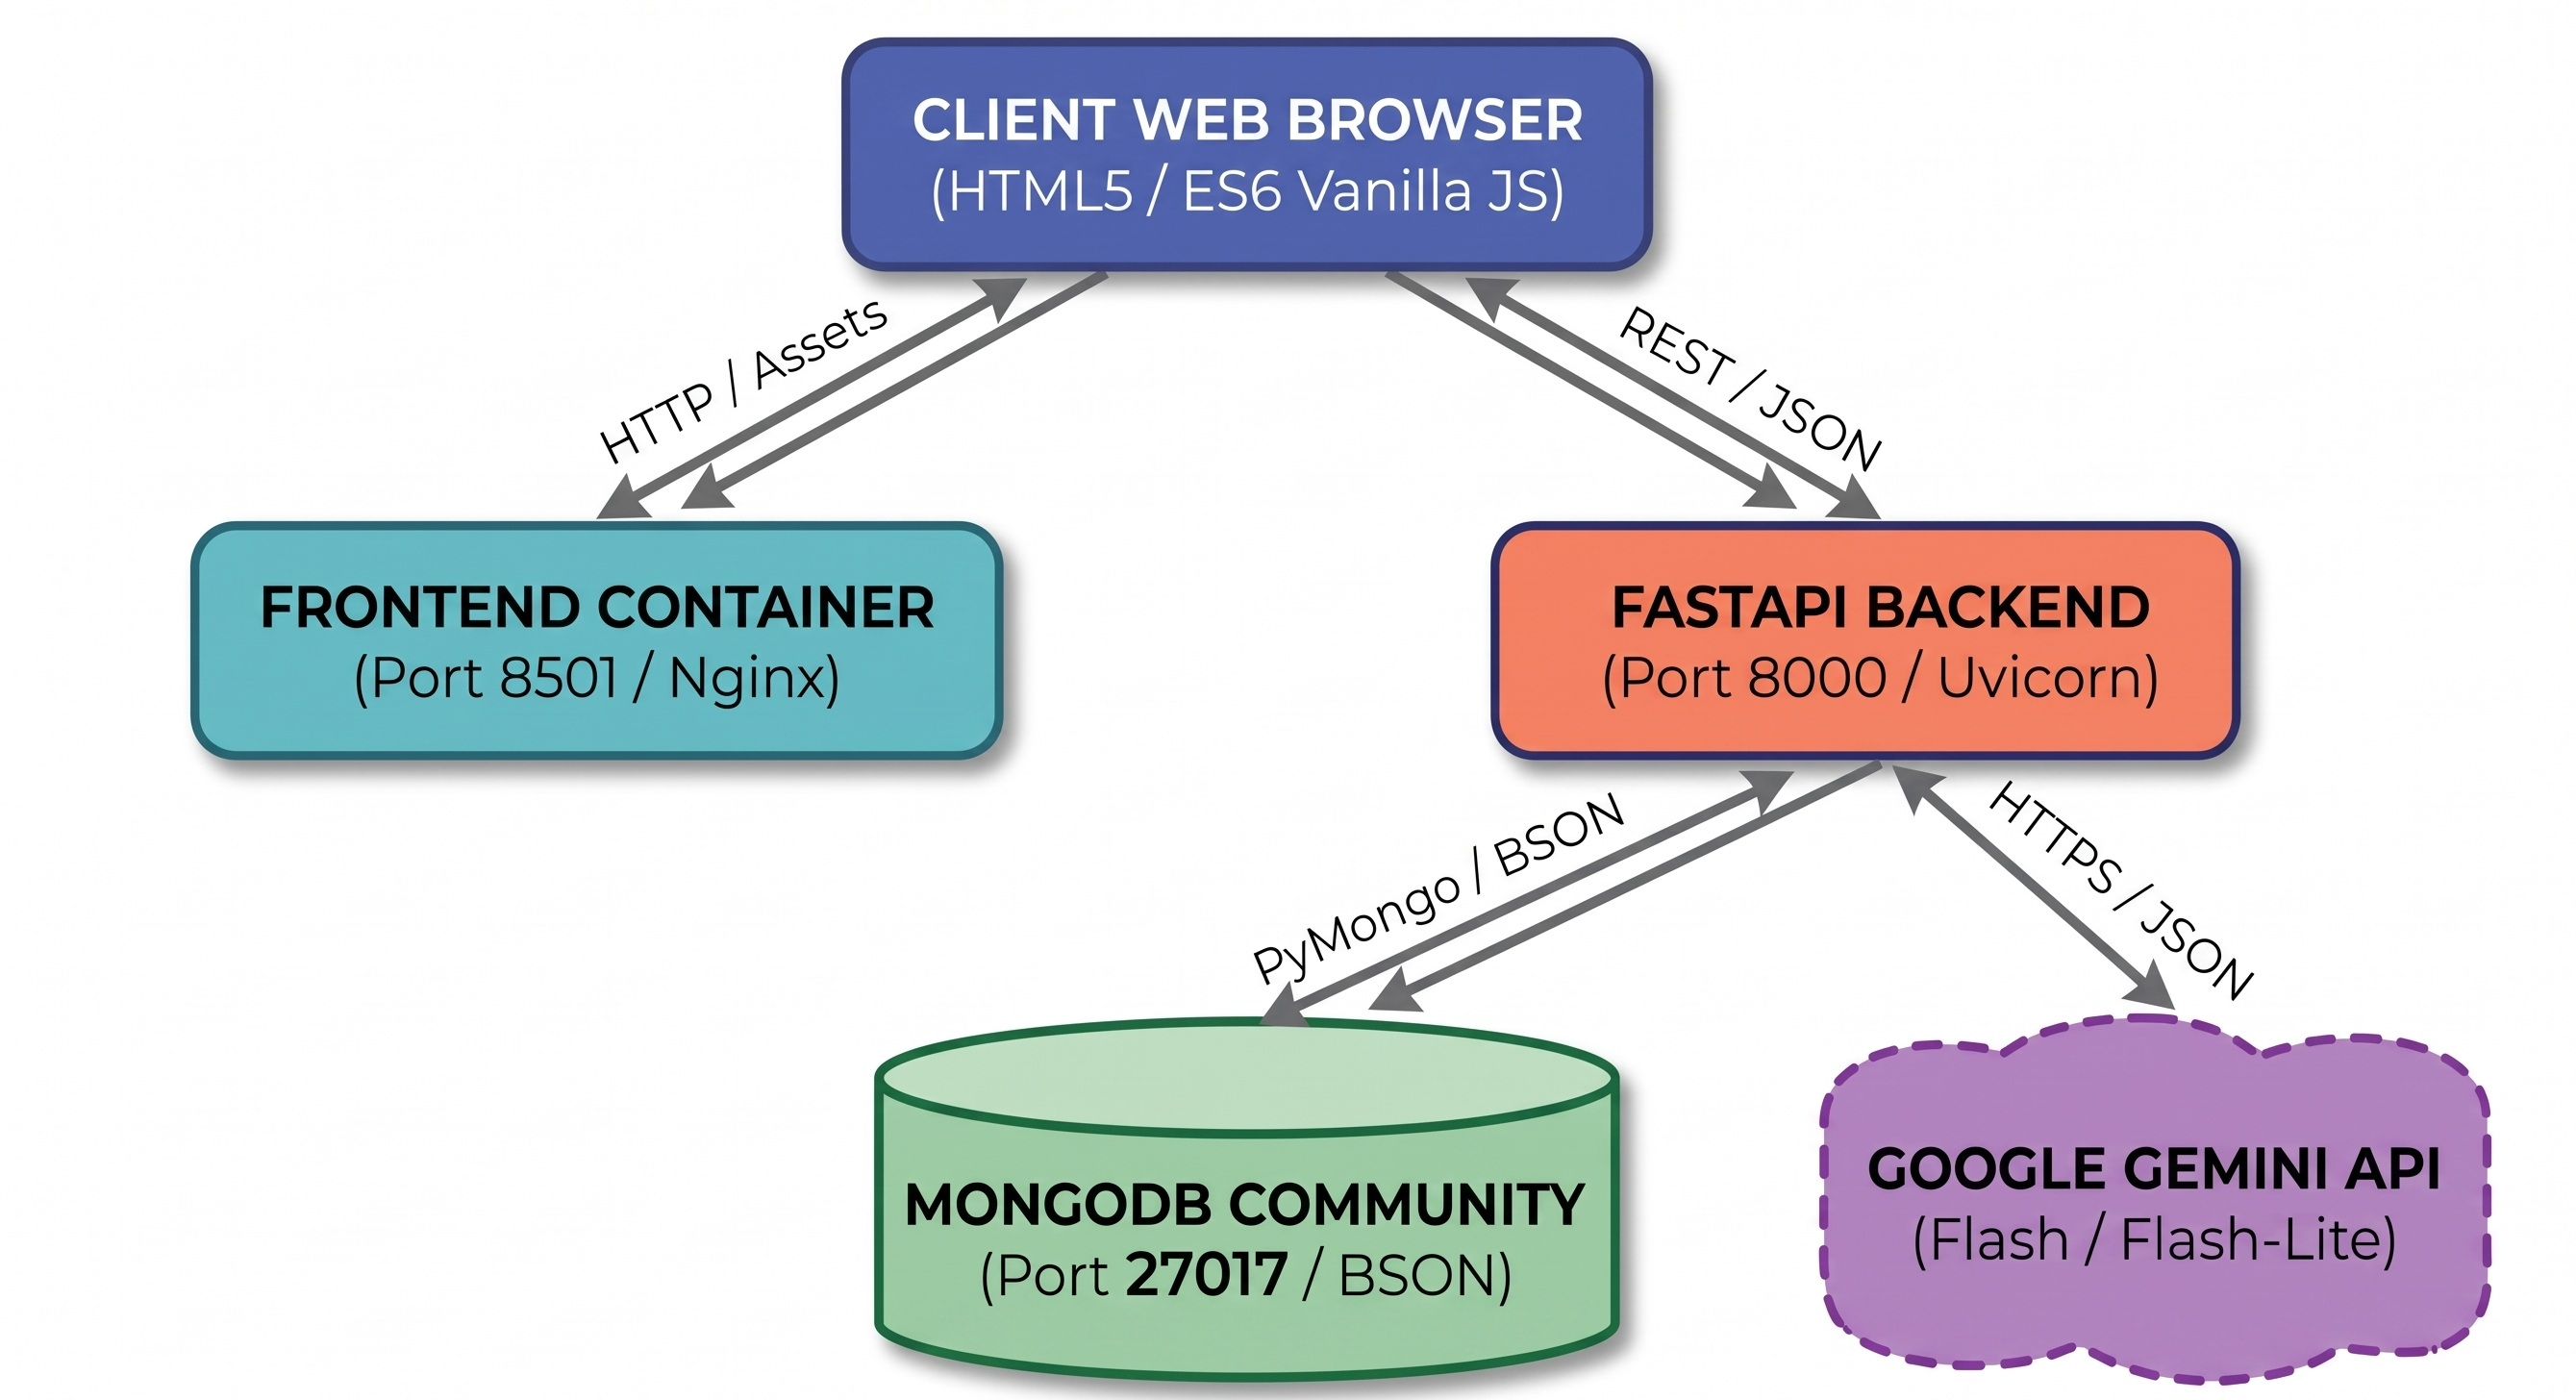
\includegraphics[width=1.0\textwidth]{images/SyncFlow_Architecture.png}
	\caption*{SyncFlow Multi-Container System Architecture and Service Topology.}
\end{figure}

\vspace{2mm}

\noindent Three services are defined in \texttt{docker-compose.yml}:
\begin{itemize}[itemsep=1pt,topsep=1pt]
    \item \textbf{Database Container (\texttt{syncflow-db})}: Runs MongoDB Community Edition (v7.0) on internal port \texttt{27017}, persisting data on a named Docker volume (\texttt{mongo\_data}) across container restarts. Container health is checked with a ping command (\texttt{mongosh --eval \allowbreak "db.\allowbreak adminCommand('ping')"});
    
    \vspace{1mm}
    
    \item \textbf{Backend Container (\texttt{syncflow-backend})}: Runs Python 3.12 with Uvicorn and FastAPI on port \texttt{8000}. It mounts the backend source directory, loads database URIs and Gemini API keys from the environment, and opens the MongoDB connection pool at startup;
    
    \vspace{1mm}
    
    \item \textbf{Frontend Container (\texttt{syncflow-frontend})}: Serves static HTML5, CSS3, and ES6 JavaScript modules on port \texttt{8501} using Python's built-in \texttt{http.server} module from the same slim image as the backend. Isolating static file delivery in its own container separates lightweight web asset serving from FastAPI's heavier schedule computations and AI calls on port \texttt{8000}, keeps page delivery running independently if the API reloads, and avoids any Node.js or bundler pipeline so plain file updates go live on browser refresh.
\end{itemize}

\newpage

\section{Database Layer and Data Integrity}
Persistence is handled through MongoDB, pairing flexible nested documents with server-side JSON Schema rules so malformed payloads cannot be written silently.

\noindent Data is stored across four core \textbf{Document Collections}:
\begin{enumerate}[leftmargin=*,itemsep=0pt,topsep=1pt,parsep=0pt]
    \item \textbf{\texttt{users}}: Account profiles, Bcrypt password hashes, administrative flags, and contributor specialty roles;
    
    \vspace{1mm}
    
    \item \textbf{\texttt{projects}}: The central project document storing metadata and governance rules, working \texttt{calendar\_settings}, nested \texttt{wbs} hierarchies, embedded \texttt{activities} (PDM links, PERT parameters, 4-tier statuses, checklists, and active timer/log entries), and saved \texttt{baselines};
    
    \vspace{1mm}
    
    \item \textbf{\texttt{teams}}: Reusable team templates created by Project Managers for import across projects;
    
    \vspace{1mm}
    
    \item \textbf{\texttt{notifications}}: System alerts, controller inspection notices, and interactive join requests.
\end{enumerate}

\vspace{4mm}

Both \texttt{users} and \texttt{projects} enforce strict MongoDB \texttt{\$jsonSchema} rules (\texttt{validationLevel=\allowbreak "strict"}) covering required fields, BSON types, and format constraints. Concurrent updates to nested activities (progress percentages, checklists, and stopwatch logs) run atomically with MongoDB \texttt{arrayFilters} and the \texttt{\$[act]} positional operator:
\begin{lstlisting}[language=Python, basicstyle=\ttfamily\scriptsize, frame=single, aboveskip=3pt, belowskip=3pt]
db.projects.update_one(
    {"_id": ObjectId(project_id)},
    {"$set": {
        "activities.$[act].status": new_status,
        "activities.$[act].actual_progress": progress
    }},
    array_filters=[{"act.activity_id": activity_id}]
)

\end{lstlisting}

Updating a single matched element in place avoids whole-document overwrites when multiple contributors work on different activities at the same time.

\vspace{6mm}

\section{Backend Architecture and Computation Engine}
The backend is written in \textbf{FastAPI} (Python 3.12) and divided into domain routers mounted under \texttt{/syncflow}. Requests and responses are checked with \textbf{Pydantic} models, passwords are salted and hashed using \textbf{Bcrypt} (\texttt{rounds=12}), and route handlers filter queries by validated user, manager, and project identifiers.

\vspace{4mm}

\noindent Recomputing CPM passes, PERT probabilities, and EVM S-curves on every read request would add unnecessary database and CPU work. Instead, \textit{SyncFlow} uses a thread-safe in-memory LRU cache backed by \texttt{collections.OrderedDict} and a reentrant \texttt{threading.Lock}:
\begin{itemize}[itemsep=0pt,topsep=1pt,parsep=0pt]
    \item \textbf{Cache Key Formulation}: Each key combines the project ID, document update timestamp, and query options: $\text{Key} = \texttt{f"\{project\_id\}:\allowbreak \{updated\_at\}:\allowbreak \{cpm\_flags\}"}$;
    \item \textbf{In-Memory Reuse}: Repeated schedule and EVM queries read directly in $O(1)$ time without hitting MongoDB;
    \item \textbf{Write Invalidation}: Every write route that edits activities, links, or calendar settings calls \texttt{invalidate\_\allowbreak project\_\allowbreak schedule\_\allowbreak cache(\allowbreak project\_id)} so stale results are dropped immediately.
\end{itemize}

\newpage

\section{RESTful API Architecture and Endpoints}
\textit{SyncFlow} exposes 55 RESTful endpoints distributed across six domain routers (\texttt{user}, \texttt{projects}, \texttt{teams}, \texttt{notifications}, \texttt{portfolio}, and \texttt{nlp}). Every endpoint validates incoming JSON payloads and query parameters through Pydantic models, returns standardized HTTP status codes (\texttt{200}, \texttt{201}, \texttt{400}, \texttt{404}), and triggers automatic schedule cache invalidation whenever underlying schedule state is mutated. To clearly distinguish the role of each service, the platform's API surface is organized below by functional domain.

\vspace{6mm}

\subsection{User Management and Authentication APIs}
User registration, credential verification, and service readiness probes are handled by the core authentication router mounted at \texttt{/syncflow/user} alongside the root health endpoint. The table below documents each user and system health API.

\vspace{4mm}

\begin{table}[H]
\centering
\small
\setlength{\tabcolsep}{5pt}
\renewcommand{\arraystretch}{1.28}
\caption*{User Account, Authentication, and System Health Endpoints.}
\vspace{-2pt}
\begin{tabularx}{\textwidth}{p{1.3cm} >{\raggedright\arraybackslash}p{6.0cm} X}
\toprule
\textbf{Verb} & \textbf{Endpoint Path} & \textbf{Functional Purpose \& Behavior} \\
\midrule
\textbf{\texttt{POST}} & \texttt{/syncflow/user/signup} & Registers a new account, validates password match and role assignment, and hashes credentials via Bcrypt (\texttt{rounds=12}). \\
\textbf{\texttt{POST}} & \texttt{/syncflow/user/login} & Authenticates username or normalized email against the stored Bcrypt digest and returns the user profile. \\
\textbf{\texttt{GET}} & \texttt{/syncflow/user} & Lists all registered workspace users to populate team selection and personnel rosters. \\
\textbf{\texttt{GET}} & \texttt{/syncflow/user/\{user\_id\}} & Fetches a single user record resolved by MongoDB \texttt{ObjectId} or normalized username. \\
\textbf{\texttt{GET}} & \texttt{/syncflow/user/\{user\_id\}/\allowbreak profile} & Returns formatted account metadata consumed by self-service profile views. \\
\textbf{\texttt{PUT}} & \texttt{/syncflow/user/\{user\_id\}} & Updates personal profile details while enforcing global uniqueness across usernames and emails. \\
\textbf{\texttt{DELETE}} & \texttt{/syncflow/user/\{user\_id\}} & Removes a user account document from the \texttt{users} collection. \\
\textbf{\texttt{GET}} & \texttt{/syncflow/health} & Lightweight liveness diagnostic confirming backend availability with an ISO UTC timestamp. \\
\bottomrule
\end{tabularx}
\end{table}

\newpage

\subsection{Project Lifecycle APIs}
Project creation, organizational governance, member discovery, and formal launch transitions are managed under \texttt{/syncflow/projects}. These routes cover project charter configuration, personnel assignments across single- and multi-team structures, Open versus Approval enrollment flows, and cross-project historical completion lookups. The table below summarizes the charter and project lifecycle endpoints.

\vspace{4mm}

\begin{table}[H]
\centering
\small
\setlength{\tabcolsep}{5pt}
\renewcommand{\arraystretch}{1.28}
\caption*{Project Charter, Governance, Discovery, and Lifecycle Endpoints.}
\vspace{-2pt}
\begin{tabularx}{\textwidth}{p{1.3cm} >{\raggedright\arraybackslash}p{6.0cm} X}
\toprule
\textbf{Verb} & \textbf{Endpoint Path} & \textbf{Functional Purpose \& Behavior} \\
\midrule
\textbf{\texttt{GET}} & \texttt{/syncflow/projects} & Lists project summaries, optionally filtered by creator \texttt{pm\_id} or participating \texttt{member\_id}. \\
\textbf{\texttt{POST}} & \texttt{/syncflow/projects} & Creates a project charter with start date, Single/Multi-Team rules, Open/Approval policies, teams, and calendar. \\
\textbf{\texttt{GET}} & \texttt{/syncflow/projects/\{project\_id\}} & Returns the complete project document including WBS, activities, dependencies, and baselines. \\
\textbf{\texttt{PUT}} & \texttt{/syncflow/projects/\{project\_id\}/\allowbreak description} & Updates the project scope statement and description in the schedule governance view. \\
\textbf{\texttt{PUT}} & \texttt{/syncflow/projects/\{project\_id\}/\allowbreak personnel} & Reassigns functional teams, Team Leads, unassigned specialists, and project Controllers. \\
\textbf{\texttt{GET}} & \texttt{/syncflow/projects/\allowbreak available/search} & Queries open or approval-gated projects by keyword and computes the user's join status. \\
\textbf{\texttt{POST}} & \texttt{/syncflow/projects/\{project\_id\}/\allowbreak join} & Enrolls a contributor immediately on Open projects or emits a join request notification on Approval projects. \\
\textbf{\texttt{POST}} & \texttt{/syncflow/projects/\{project\_id\}/\allowbreak kickoff} & Formally initiates project execution, transitioning lifecycle status from planning to active state. \\
\textbf{\texttt{GET}} & \texttt{/syncflow/projects/\allowbreak completed-activities} & Aggregates Controller-verified historical activities across projects for cross-project reference. \\
\textbf{\texttt{DELETE}} & \texttt{/syncflow/projects/\{project\_id\}} & Deletes a project record from MongoDB and evicts any cached schedule artifacts. \\
\bottomrule
\end{tabularx}
\end{table}

\newpage

\subsection{Schedule Planning, Sequencing, and Operations Research APIs}
The core scheduling endpoints manage hierarchical Work Breakdown Structure assembly, precedence network validation, deterministic CPM/PERT calculation, baseline locking, and defense-grade quality auditing. Whenever structural or temporal data change, the backend automatically evicts stale entries from the LRU schedule cache. The table below details these endpoints. 

\vspace{4mm}

\begin{table}[H]
\centering
\small
\setlength{\tabcolsep}{5pt}
\renewcommand{\arraystretch}{1.28}
\caption*{Work Breakdown, Precedence Sequencing, CPM/PERT Analytics, and Audit Endpoints.}
\vspace{-2pt}
\begin{tabularx}{\textwidth}{p{1.3cm} >{\raggedright\arraybackslash}p{6.0cm} X}
\toprule
\textbf{Verb} & \textbf{Endpoint Path} & \textbf{Functional Purpose \& Behavior} \\
\midrule
\textbf{\texttt{PUT}} & \texttt{/syncflow/projects/\{project\_id\}/\allowbreak wbs} & Replaces or updates the hierarchical WBS tree (Major Deliverables, Sub-deliverables, and Work Packages). \\
\textbf{\texttt{PUT}} & \texttt{/syncflow/projects/\{project\_id\}/\allowbreak deliverables} & Compatibility route mapping legacy deliverable arrays onto the canonical nested \texttt{wbs} structure. \\
\textbf{\texttt{PUT}} & \texttt{/syncflow/projects/\{project\_id\}/\allowbreak activities} & Persists discrete activities, milestones, PERT inputs, and resource assignees. \\
\textbf{\texttt{GET}} & \texttt{/syncflow/projects/\{project\_id\}/\allowbreak schedule-health} & Inspects the activity graph for open ends, dangling activities, excessive lags, logic density, and cycles. \\
\textbf{\texttt{PUT}} & \texttt{/syncflow/projects/\{project\_id\}/\allowbreak dependencies} & Updates directed PDM precedence links (\texttt{FS}, \texttt{SS}, \texttt{FF}, \texttt{SF}), rejecting negative lags and cyclic loops. \\
\textbf{\texttt{POST}} & \texttt{/syncflow/projects/\{project\_id\}/\allowbreak schedule-settings} & Saves externally imposed deadlines, near-critical float thresholds, and default diagram mode (\texttt{aon}/\texttt{aoa}). \\
\textbf{\texttt{GET}} & \texttt{/syncflow/projects/\{project\_id\}/\allowbreak schedule} & Executes cached CPM passes, computing early/late dates, Total/Free/Project Float, and AON/AOA graph payloads. \\
\textbf{\texttt{GET}} & \texttt{/syncflow/projects/\{project\_id\}/\allowbreak pert-analysis} & Computes Critical Path expected duration ($\mu_{CP}$), variance ($\sigma_{CP}^2$), $Z$-score, and completion probability $\Phi(Z)$. \\
\textbf{\texttt{POST}} & \texttt{/syncflow/projects/\{project\_id\}/\allowbreak baselines} & Freezes the calculated CPM schedule into the canonical Planned Baseline snapshot for variance tracking. \\
\textbf{\texttt{GET}} & \texttt{/syncflow/projects/\{project\_id\}/\allowbreak baselines} & Retrieves stored Planned Baseline snapshots for planned-versus-actual schedule comparison. \\
\textbf{\texttt{DELETE}} & \texttt{/syncflow/projects/\{project\_id\}/\allowbreak baselines/\{baseline\_id\}} & Clears the saved baseline snapshot when major scope replanning is approved. \\
\textbf{\texttt{GET}} & \texttt{/syncflow/projects/\{project\_id\}/\allowbreak schedule/dcma-quality} & Audits the schedule against all 14 DCMA metrics, returning compliance scores, grade (\texttt{A--F}), and culprits. \\
\bottomrule
\end{tabularx}
\end{table}

\newpage

\subsection{Schedule Control, Live Time Tracking, and Enterprise APIs}
Live execution monitoring, Earned Value tracking, and granular Trello-style stopwatch logging operate directly against nested activity records using atomic MongoDB updates. The table below details the schedule control and activity time-tracking endpoints.

\vspace{4mm}

\begin{table}[H]
\centering
\small
\setlength{\tabcolsep}{5pt}
\renewcommand{\arraystretch}{1.28}
\caption*{Schedule Control, Earned Value, and Activity Stopwatch Timer Endpoints.}
\vspace{-2pt}
\begin{tabularx}{\textwidth}{p{1.3cm} >{\raggedright\arraybackslash}p{6.0cm} X}
\toprule
\textbf{Verb} & \textbf{Endpoint Path} & \textbf{Functional Purpose \& Behavior} \\
\midrule
\textbf{\texttt{GET}} & \texttt{/syncflow/projects/\{project\_id\}/\allowbreak control-schedule} & Computes Earned Value KPIs ($PV$, $EV$, $SV$, $SPI$, $EAC_t$), status distributions, and S-Curve Banana Envelope points. \\
\textbf{\texttt{PUT}} & \texttt{/syncflow/projects/\{project\_id\}/\allowbreak activities/\{activity\_id\}/\allowbreak status} & Transitions execution state (Not Started, WIP, Completed, Verified), logs deliverable evidence, and records Controller sign-off. \\
\textbf{\texttt{POST}} & \texttt{/syncflow/projects/\{project\_id\}/\allowbreak activities/seed-progress} & Initializes realistic benchmark progress across activities for simulation and testing scenarios. \\
\textbf{\texttt{POST}} & \texttt{/syncflow/projects/\{project\_id\}/\allowbreak activities/\{activity\_id\}/\allowbreak timer/start} & Starts an active stopwatch session bound strictly to an activity currently in Work-in-Progress state. \\
\textbf{\texttt{POST}} & \texttt{/syncflow/projects/\{project\_id\}/\allowbreak activities/\{activity\_id\}/\allowbreak timer/stop} & Stops the active stopwatch, computes elapsed seconds, writes a persistent log, and emits state alerts if needed. \\
\textbf{\texttt{GET}} & \texttt{/syncflow/projects/\{project\_id\}/\allowbreak activities/\{activity\_id\}/\allowbreak time-logs} & Retrieves the full chronological timer history and cumulative duration recorded for one activity. \\
\textbf{\texttt{GET}} & \texttt{/syncflow/projects/\{project\_id\}/\allowbreak time-logs/summary} & Summarizes total logged work hours across every project activity for executive time auditing. \\
\textbf{\texttt{PUT}} & \texttt{/syncflow/projects/\{project\_id\}/\allowbreak activities/\{activity\_id\}/\allowbreak time-logs/\{log\_id\}} & Modifies elapsed duration or session notes on a user-created time log entry. \\
\textbf{\texttt{DELETE}} & \texttt{/syncflow/projects/\{project\_id\}/\allowbreak activities/\{activity\_id\}/\allowbreak time-logs/\{log\_id\}} & Removes an erroneous time log entry and recalculates the activity's accumulated effort. \\
\textbf{\texttt{GET}} & \texttt{/syncflow/projects/\{project\_id\}/\allowbreak my-time-logs} & Returns all work sessions logged by a single contributor across every activity in the project. \\
\bottomrule
\end{tabularx}
\end{table}

\newpage

\noindent Cross-project administration, reusable organizational teams, portfolio analytics, and interactive alerts are exposed through dedicated routers (\texttt{/syncflow/teams}, \texttt{/syncflow/portfolio}, and \texttt{/syncflow/notifications}). The table below summarizes these enterprise coordination APIs.

\begin{table}[H]
\centering
\footnotesize
\setlength{\tabcolsep}{5pt}
\renewcommand{\arraystretch}{1.28}
\caption*{Reusable Teams Library, Executive Portfolio, and Notification Hub Endpoints.}
\vspace{-2pt}
\begin{tabularx}{\textwidth}{p{1.3cm} >{\raggedright\arraybackslash}p{6.0cm} X}
\toprule
\textbf{Verb} & \textbf{Endpoint Path} & \textbf{Functional Purpose \& Behavior} \\
\midrule
\textbf{\texttt{GET}} & \texttt{/syncflow/teams} & Retrieves saved organizational team templates filtered optionally by creator \texttt{pm\_id}. \\
\textbf{\texttt{POST}} & \texttt{/syncflow/teams} & Upserts a custom team template (name, roster IDs, and Team Lead) into the global library. \\
\textbf{\texttt{GET}} & \texttt{/syncflow/portfolio/dashboard} & Aggregates multi-project Earned Value KPIs ($PV$, $EV$, $SV$, $SPI$) and critical slippage indicators. \\
\textbf{\texttt{POST}} & \texttt{/syncflow/notifications} & Creates a targeted or project-wide notification entry in the \texttt{notifications} collection. \\
\textbf{\texttt{GET}} & \texttt{/syncflow/notifications} & Fetches notifications addressed to a \texttt{user\_id}, with optional \texttt{project\_id} scoping. \\
\textbf{\texttt{GET}} & \texttt{/syncflow/notifications/\allowbreak unread-count} & Returns the unread notification counter used to update navigation badges in real time. \\
\textbf{\texttt{PUT}} & \texttt{/syncflow/notifications/\allowbreak \{notification\_id\}/read} & Appends the requesting user to the notification's \texttt{read\_by} array. \\
\textbf{\texttt{PUT}} & \texttt{/syncflow/notifications/\allowbreak mark-all-read} & Marks all visible notifications for the user as read in a single batch operation. \\
\textbf{\texttt{POST}} & \texttt{/syncflow/notifications/\allowbreak \{notification\_id\}/action} & Resolves interactive requests (such as approving or rejecting project join applications). \\
\textbf{\texttt{DELETE}} & \texttt{/syncflow/notifications/\allowbreak \{notification\_id\}} & Soft-deletes a notification for the caller by recording their ID in \texttt{deleted\_by}. \\
\bottomrule
\end{tabularx}
\end{table}

\vspace{4mm}

\subsection{Natural Language Processing and AI Service APIs}
Natural Language Processing capabilities are exposed via the \texttt{/syncflow/nlp} and \texttt{/syncflow/\allowbreak projects/\allowbreak \{project\_id\}/\allowbreak nlp} endpoints, turning unstructured scope descriptions and workflow prose into schema-validated project structures. The table below documents the NLP endpoints examined further in Chapter 5.

\begin{table}[H]
\centering
\footnotesize
\setlength{\tabcolsep}{5pt}
\renewcommand{\arraystretch}{1.28}
\caption*{Natural Language Processing, Key Verification, and Schedule Extraction Endpoints.}
\vspace{-2pt}
\begin{tabularx}{\textwidth}{p{1.3cm} >{\raggedright\arraybackslash}p{6.0cm} X}
\toprule
\textbf{Verb} & \textbf{Endpoint Path} & \textbf{Functional Purpose \& Behavior} \\
\midrule
\textbf{\texttt{GET}} & \texttt{/syncflow/nlp/models} & Returns the strictly permitted Gemini Flash model identifiers configured by the backend. \\
\textbf{\texttt{POST}} & \texttt{/syncflow/nlp/verify-key} & Tests whether a user-supplied or environment API key authenticates cleanly with active models. \\
\textbf{\texttt{POST}} & \texttt{/syncflow/projects/\{project\_id\}/\allowbreak nlp/text-to-wbs} & Parses unstructured project scope into a multi-tier WBS and PERT-initialized activities (\texttt{merge} or \texttt{replace}). \\
\textbf{\texttt{POST}} & \texttt{/syncflow/projects/\{project\_id\}/\allowbreak nlp/estimate-durations} & Evaluates activity texts semantically to infer DCMA-compliant $(a, m, b)$ estimates and risk rationales. \\
\textbf{\texttt{POST}} & \texttt{/syncflow/projects/\{project\_id\}/\allowbreak nlp/extract-dependencies} & Extracts directed PDM precedence links (\texttt{FS}, \texttt{SS}, \texttt{FF}, \texttt{SF}) and non-negative lags from narratives with cycle checks. \\
\bottomrule
\end{tabularx}
\end{table}

\newpage

\section{Frontend Architecture and Data Visualizations}
\subsection{Interactive Network Visualizations via Vis-Network}
After moving away from the initial Streamlit prototype, the frontend was rebuilt in plain Vanilla JavaScript, HTML5, and custom CSS (\texttt{styles.css}). Keeping the client free of bundlers and heavy UI frameworks keeps pages fast to load and makes direct DOM updates straightforward during interactive graph edits.

\vspace{2mm}

\noindent \textit{SyncFlow} uses the \texttt{vis-network} canvas library for three network diagrams:
\begin{enumerate}[leftmargin=*,itemsep=1pt,topsep=1pt]
    \item \textbf{Hierarchical WBS Tree}: Top-down tree layout ($UD$) tracing the breakdown from the root project through Major Deliverables, sub-deliverables, and terminal Work Packages;
    
    \vspace{1mm}
    
    \item \textbf{Horizontal PDM Precedence Canvas}: Left-to-right directed graph ($LR$) color-coding dependency types: FS (Blue), SS (Purple), FF (Teal), and SF (Dashed amber);
    
    \vspace{1mm}
    
    \item \textbf{AON and AOA Network Graphs}: In the Develop Schedule Process view, the canvas switches between Activity-on-Node blocks (showing early/late dates and float values, with the Critical Path marked in red) and Activity-on-Arrow PERT event graphs with dual-moment circles and dashed dummy links.
\end{enumerate}

\vspace{4mm}

\subsection{Earned Value S-Curve Visualization via Chart.js}
In the \textbf{Control Schedule dashboard}, \textit{SyncFlow} renders the time-based EVM S-Curve with \texttt{Chart.js}. The chart plots Early Planned Value ($PV_{\text{Early}}$) and Late Planned Value ($PV_{\text{Late}}$) to form the Banana Envelope alongside Actual Earned Value ($EV$) and the EAC projection, making schedule drift easy to spot at a glance.

\vspace{4mm}

\subsection{Client-Side Event Bus and State Synchronization}
\textbf{Client state} is handled by modular dashboard scripts without external state libraries such as Redux. Page scripts listen for user interactions (node dragging, duration edits, modal submissions), send targeted REST calls, and refresh the DOM from the response. Users receive brief toast alerts after actions, while confirmation dialogs guard destructive steps such as baseline resets or activity deletions.
